\documentclass{article}
\usepackage{graphicx}
\usepackage{tikz}
\usepackage{amsmath}
\usetikzlibrary{positioning} 
\usetikzlibrary{shapes}
\usepackage{hyperref}
\usepackage{geometry}

\geometry{a4paper, margin=1in}

\title{Final Project Report}
\author{Muchammad Daniyal Kautsar}
\date{}

\begin{document}

\maketitle
\vspace{-3em}
\begin{center}
    21/479067/TK/52800
\end{center}
\vspace{-1.5em}
\begin{center}
    TIF5113 Software Architecture
\end{center}

\section{Introduction}

We present the architectural design and motivation behind implementing a robust, scalable microservices-based system. The system comprises three primary services: \textbf{User Service}, \textbf{Catalog Service}, and \textbf{Order Service}, each performing distinct roles to manage user accounts, book inventories, and order processes, respectively. We employ modern tools and practices to ensure high availability, scalability, and maintainability.

\section{System Architecture}

\subsection{Microservices Architecture}

The system is designed using a \textbf{microservices architecture}, which decomposes the application into smaller, independent services. Each service is responsible for a specific business capability and communicates with others through well-defined APIs.

\subsection{Key Components}

\subsubsection{User Service}
\begin{itemize}
    \item \textbf{Functionality}: Manages user accounts and authentication.
    \item \textbf{Technology}: Python (Flask), MongoDB.
    \item \textbf{API Endpoints}:
    \begin{itemize}
        \item \texttt{POST /register}: Register a new user.
        \item \texttt{POST /login}: Authenticate a user.
    \end{itemize}
\end{itemize}

\subsubsection{Catalog Service}
\begin{itemize}
    \item \textbf{Functionality}: Handles the inventory of books.
    \item \textbf{Technology}: Python (Flask), MongoDB, Redis (for caching).
    \item \textbf{API Endpoints}:
    \begin{itemize}
        \item \texttt{POST /books}: Add a new book to the catalog.
        \item \texttt{GET /books}: Retrieve the list of books.
        \item \texttt{GET /books/\{id\}}: Retrieve details of a specific book.
    \end{itemize}
\end{itemize}

\subsubsection{Order Service}
\begin{itemize}
    \item \textbf{Functionality}: Manages the order process.
    \item \textbf{Technology}: Python (Flask), MongoDB.
    \item \textbf{API Endpoints}:
    \begin{itemize}
        \item \texttt{POST /order}: Place a new order.
        \item \texttt{GET /orders/\{username\}}: Retrieve orders for a specific user.
    \end{itemize}
\end{itemize}

\subsection{Supporting Components}

\subsubsection{Nginx Gateway}
\begin{itemize}
    \item \textbf{Role}: Acts as a reverse proxy, routing incoming requests to the appropriate service based on URL paths.
    \item \textbf{Ports}:
    \begin{itemize}
        \item \texttt{5000}: Gateway entry point.
        \item \texttt{5001-5003}: Service-specific ports.
    \end{itemize}
\end{itemize}

\subsubsection{MongoDB}
\begin{itemize}
    \item \textbf{Role}: Stores persistent data for user accounts, books, and orders.
    \item \textbf{Instances}:
    \begin{itemize}
        \item \texttt{userdb}: User data.
        \item \texttt{catalogdb}: Book data.
        \item \texttt{orderdb}: Order data.
    \end{itemize}
\end{itemize}

\subsubsection{Redis}
\begin{itemize}
    \item \textbf{Role}: Provides caching to enhance the performance of the Catalog Service.
\end{itemize}

\subsubsection{Docker}
\begin{itemize}
    \item \textbf{Role}: Containerization and node replication via Docker Swarm for ensuring low downtime, higher availability and scalability.
\end{itemize}

\section{Motivation}
\begin{itemize}
    \item \textbf{Modularity and Maintainability:} Independent development, deployment, and scaling of services simplifies management and adaptation to changes.
    \item \textbf{Scalability:} Individual services can be scaled based on their specific load, ensuring efficient resource allocation.
    \item \textbf{Fault Isolation:} Failure of one service does not impact the entire system, maintaining service availability.
    \item \textbf{Technology Agility:} Each service can leverage the most suitable technologies, enabling optimal performance and flexibility.
    \item \textbf{Continuous Deployment:} Regular updates to services are possible without disrupting the overall system, supporting modern DevOps practices.
    \item \textbf{High Availability:} Docker Swarm enables replication and redundancy, ensuring the system can handle failures gracefully. 
\end{itemize}

\newpage
\section*{Appendix}
\subsection*{Code Repositories}
All of the code repositories can be found at \href{https://github.com/mdaniyalk/final-apl}{github}.

\subsection*{System Architecture Overview}

\begin{figure}[h]
    \centering
    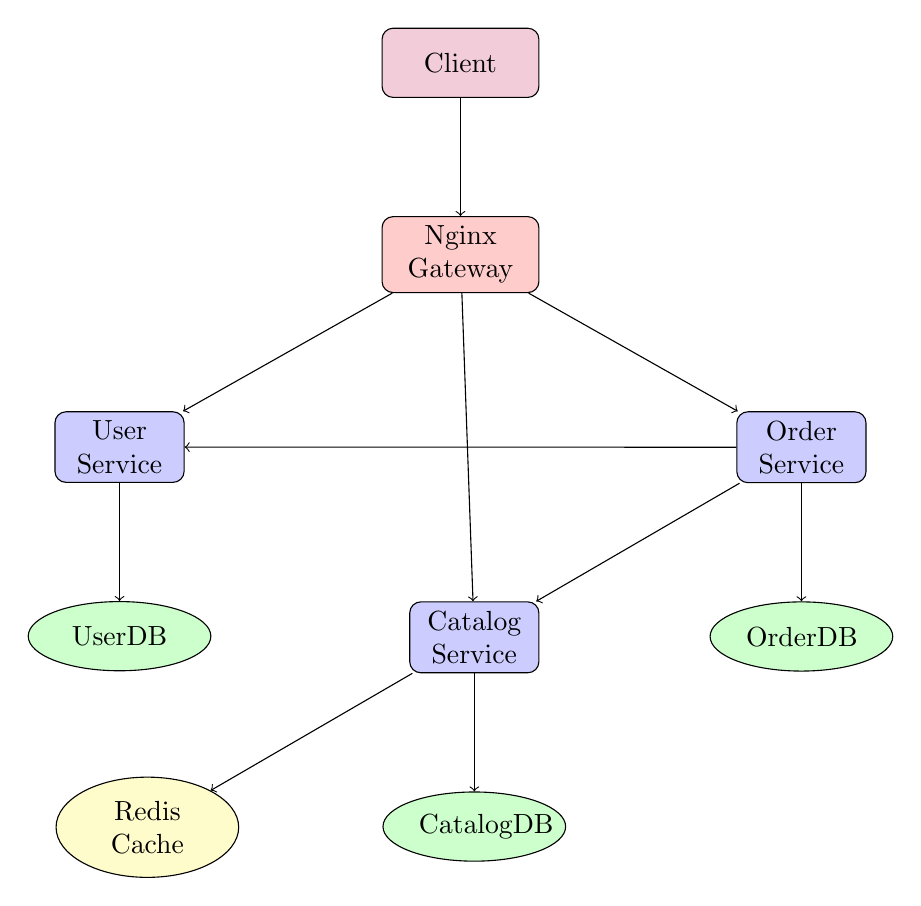
\begin{tikzpicture}[
        node distance=1.5cm and 2.5cm,
        process/.style={rectangle, draw, fill=blue!20, text width=4em, text centered, rounded corners, minimum height=2.5em},
        data/.style={ellipse, draw, fill=green!20, text width=4em, text centered, minimum height=2.5em},
        cache/.style={ellipse, draw, fill=yellow!20, text width=4em, text centered, minimum height=2.5em},
        gateway/.style={rectangle, draw, fill=red!20, text width=5em, text centered, rounded corners, minimum height=2.5em},
        user/.style={rectangle, draw, fill=purple!20, text width=5em, text centered, rounded corners, minimum height=2.5em}
    ]
       
        \node[user] (client) {Client};
        \node[gateway, below=of client] (nginx) {Nginx Gateway};
        \node[process, below right=of nginx] (order) {Order Service};
        \node[process, below left=of nginx] (user) {User Service};
        \node[process, below left=of order] (catalog) {Catalog Service};
        
        \node[data, below=of user] (userdb) {UserDB};
        \node[data, below=of catalog] (catalogdb) {CatalogDB};
        \node[data, below=of order] (orderdb) {OrderDB};
        \node[cache,below left=of catalog] (redis) {Redis Cache};

       
        \draw[->] (client) -- (nginx);
        \draw[->] (nginx) -- (user);
        \draw[->] (nginx) -- (catalog);
        \draw[->] (nginx) -- (order);
        \draw[->] (user) -- (userdb);
        \draw[->] (catalog) -- (catalogdb);
        \draw[->] (catalog) -- (redis);
        \draw[->] (order) -- (orderdb);
        \draw[->] (order) -- (user);
        \draw[->] (order) -- (catalog);
    \end{tikzpicture}
    \caption{System Architecture Overview}
    \label{fig:system-architecture}
\end{figure}

\end{document}
